\subsection{Die Reellen Zahlen}
Symbol: $\mathbb{R}$\\
sind alle Rationalen und irrationalen Zahlen

\hfill \break
Intervale beschreiben einen Zahlenbereich: $\{[1,2];[1.2,3.4]\}$


\hfill \break
\begin{tikzpicture}
    \draw (0,0) -- (4,0);
    \foreach \X in {1,...,3}
    \draw (\X,0.1) -- (\X,-0.1);
    \foreach \X in {1,3}
    \node[anchor=north] at (\X,-0.1){\X};
\end{tikzpicture}

\hfill \break
Zwischen 1 und 3 Liegen unendlich viele Zahlen


\hfill \break
Schreibweisen von Intervalen:
\begin{itemize}
    \item $[1,2]$ = Geschlossener Interval
    \item $[1,2) = [1,2[$ = Halboffener Interval
    \item $(1,2] = ]1,2]$ = Halboffener Interval
    \item $(1,2) = ]1,2[$ = Offener Interval
\end{itemize}



\hfill \break
Beschreibungen:
\begin{center}
    \begin{tabular}{ |c|c|c| }
        \hline
        Aufzählend             & Grafisch                                      & Beschreibend     \\
        A = $\{2,3,4,5\} $     & 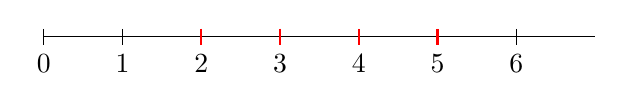
\begin{tikzpicture}
                                     \draw (0,0) -- (7,0);
                                     \foreach \X in {0,...,6}
                                     \draw (\X,0.1) -- (\X,-0.1);
                                     \foreach \X in {0,...,6}
                                     \node[anchor=north] at (\X,-0.1){\X};
                                     \foreach \X in {2,3,4,5}
                                     \draw[color=red,thick] (\X,0.1) -- (\X,-0.1);
                                 \end{tikzpicture} & A = $\{x \in \mathbb{N} | 2 \leq x \leq 5\}$ \\
        B = $\{-2,-1,0,1,2\} $ & 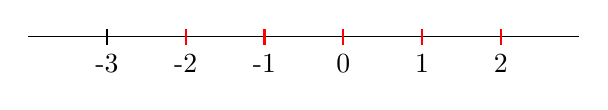
\begin{tikzpicture}
                                     \draw (-4,0) -- (3,0);
                                     \foreach \X in {-3,...,2}
                                     \draw (\X,0.1) -- (\X,-0.1);
                                     \foreach \X in {-3,...,2}
                                     \node[anchor=north] at (\X,-0.1){\X};
                                     \foreach \X in {-2,...,2}
                                     \draw[color=red,thick] (\X,0.1) -- (\X,-0.1);
                                 \end{tikzpicture} & B = $\{x \in \mathbb{Z} |-2 \leq x < 2\}$    \\
        C = $[-1,3]$           & 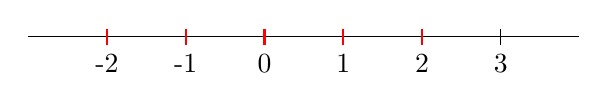
\begin{tikzpicture}
                                     \draw (-3,0) -- (4,0);
                                     \foreach \X in {-2,...,3}
                                     \draw (\X,0.1) -- (\X,-0.1);
                                     \foreach \X in {-2,...,3}
                                     \node[anchor=north] at (\X,-0.1){\X};
                                     \foreach \X in {-2,...,2}
                                     \draw[color=red,thick] (\X,0.1) -- (\X,-0.1);
                                 \end{tikzpicture} & C = $\{x \in \mathbb{R} |-1 \leq x < 3\}$    \\
        D = $]2,5]$            & 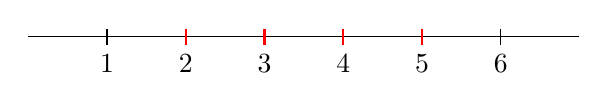
\begin{tikzpicture}
                                     \draw (0,0) -- (7,0);
                                     \foreach \X in {1,...,6}
                                     \draw (\X,0.1) -- (\X,-0.1);
                                     \foreach \X in {1,...,6}
                                     \node[anchor=north] at (\X,-0.1){\X};
                                     \foreach \X in {2,...,5}
                                     \draw[color=red,thick] (\X,0.1) -- (\X,-0.1);
                                 \end{tikzpicture} & D = $\{x \in \mathbb{R} | 2 < x \leq 5\}$    \\
        \hline
    \end{tabular}
\end{center}